
\begin{frame}
  \frametitle{Какво е качествен код ?}

\begin{exampleblock}{}
  {\large ``Качеството е форма и функция.  Кодът трябва да функционира така, както очавкам, когато гo използвам.''}
%  \vskip5mm
%  \hspace*\fill{\small--- IKEA Catalog, 2017}
\end{exampleblock}
\end{frame}

\begin{frame}
   \begin{center}
   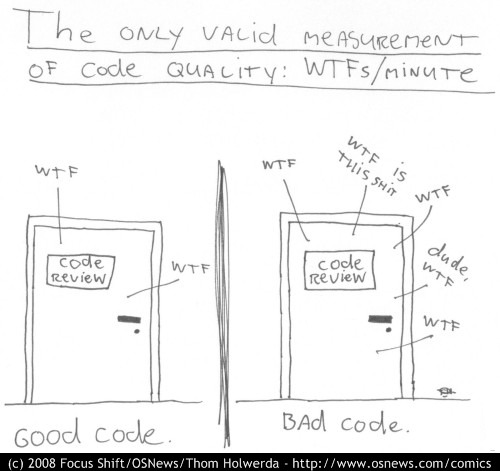
\includegraphics[width=\textwidth,height=0.8\textheight,keepaspectratio]{wtfm.jpg}
   \end{center}
\end{frame}

\begin{frame}
  \frametitle{Лош код}
  Причини:
  \begin{itemize}
  \item Няма време
  \item Симптом на счупеният прозорец
  \item Прекалена индирекция
  \item Лош дизайн
  \item Липса на умения
  \item Липса на специализирани знания
  \item Неосъзнаване на проблема
  \end{itemize}
\end{frame}

\begin{frame}
  \frametitle{Почистване на лош код}
  \begin{minipage}[t]{0.48\linewidth}
    \begin{itemize}
        \item Крие рискове
        \item Отнема време
        \item Необоходимост
    \end{itemize}
  \end{minipage}\hfill
  \begin{minipage}[t]{0.48\linewidth}
      \begin{itemize}
          \item Version Control
          \item Test Suite
      \end{itemize}
  \end{minipage}
\end{frame}


%\begin{frame}
%  \frametitle{Пример 1}
%  Качествения код е лесен за:
%  \begin{itemize}
%  \item разбиране от хора
%  \item развиване
%  \item поддръжка
%  \end{itemize}
%\end{frame}


%\begin{frame}
%  \frametitle{Пример 2: GotoBLAS}
%  Качествения код:
%  \begin{itemize}
%  \item оптимизиран до максимум
%  \item за специализиран процесор
%  \item асемблер
%  \end{itemize}
%\end{frame}


%\begin{frame}
%  \frametitle{Пример 3: Sparse Suite}
%  Качествения код:
%  \begin{itemize}
%  \item разнообразни алгоритми
%  \item високопроизводителен
%  \item минимални дефекти
%  \end{itemize}
%\end{frame}


%\begin{frame}
%  \frametitle{Sparse Suite}
%  MATLAB: $A \vec{x} = \vec{b}$ 
%  \begin{itemize}
%  \item 120,000 линий код (C / C++) 
%  \item 11 дни -> 7 минути
%  \item 3 дефекта за 15 години
%  \item 3 пъти по-надежден от NASA
%  \end{itemize}
%\end{frame}
